\documentclass[a4paper]{article}
\usepackage[utf8]{inputenc}
\usepackage{amsmath}
\usepackage{amsfonts}
\usepackage{authblk}
%\usepackage{dblfloatfix}
\usepackage{hyperref}
\usepackage{graphicx}
\usepackage{minted}
\usepackage[numbers,square]{natbib}
\usepackage{xcolor}
\usepackage{xspace}
\usepackage{url}
\usepackage{magazine-style}

\definecolor{rulecolor}{rgb}{0.80,0.80,0.80}
\newminted{python}{frame=single,rulecolor=\color{rulecolor}}


\title{Scikit-learn: machine learning without learning the machinery}

\author{The authors}


\begin{document}

\maketitle

\begin{abstract}
Machine learning is a pervasive development at the intersection of
statistics and computer science. While it can benefit many
data-related applications, the technicality of the research literature
and the corresponding algorithms slows down its adoption. Scikit-learn is
a open-source software project that aims to make machine learning
accessible to all, whether it be in academia or in the industry. It
benefits from 
the general-purpose Python language, that enjoys a huge growth in
the scientific world, as well as a striving ecosystem of contributors.
Here we give a quick introduction to scikit-learn as well as to
machine-learning basics.
\end{abstract}

\section{A software project across communities}

\paragraph{Project vision}
%
Scikit-learn was born from the observation that most standard
machine-learning algorithms were out of reach of the users that could
most benefit from them: researchers --biologists, climate
scientists, experimental physicists-- or developers --for web
services or domain-specific applications.
%
Implementations mostly consisted of scattered piece of code to download
on researchers' web pages, with the notable exception of
statistic-specific environments such as the R language \cite{Rmanual}, or
the Weka java library \cite{hall2009weka}.

Scikit-learn aims to bridge the gap between machine-learning research and
applications by providing a library, and not an environment, in a
general-purpose language, relying on domain-agnostic data structures
\cite{pedregosa2011}. Emphasis is put on quality and ease of use, which
implies focus on installation issues, documentation, and API design
\cite{buitinck2013ecml}. For the project to be usable in real-world
settings, computational performance is also a priority.

\paragraph{The Python data ecosystem}
%
Machine learning is only a small part of a data-analysis pipeline, and
scikit-learn nicely dovetails into the rich Python ecosystem: scientific
and numeric tools \cite{oliphant2007python,varoquaux2013scipy}, but also
text processing tools, web servers...
%
For its numerical needs, scikit-learn leverages NumPy arrays
\cite{vanderwalt2011} --data structures for efficient numerical
computation--, SciPy --a collection of classic numerical algorithms--,
matplotlib \cite{hunter2007matplotlib} --for scientific plotting-- and
Cython, to generate and call compiled code in a Python-like syntax
\cite{behnel2011cython}.
%
A plethora of Python packages can help users with input or preprocessing
of data, notably Pandas for columnar data \cite{mckinney2012}, scikit-image
for images, and NLTK for text. Finally, the IPython environment
\cite{perez2007ipython} is priceless for interactive work.

\paragraph{Some history}
%
Scikit-learn started circa 2007 as code from David Cournapeau and
Matthieu Brucher's PhD work, but dwindled down till 2010, year at which the
Parietal team from INRIA adopted the project, hiring a full time
engineer. Basics API were defined and an efficient binding of LibSVM
\cite{chang2011libsvm} gave the project a compelling advantage. In
December 2011, the first international sprint was organized with generous
funding from Google. Today, the project has grown vastly beyond
INRIA into a worldwide open source effort.

\section{A brief introduction to machine learning}

\begin{figure}[b]
    %\hspace*{-.015\linewidth}%
    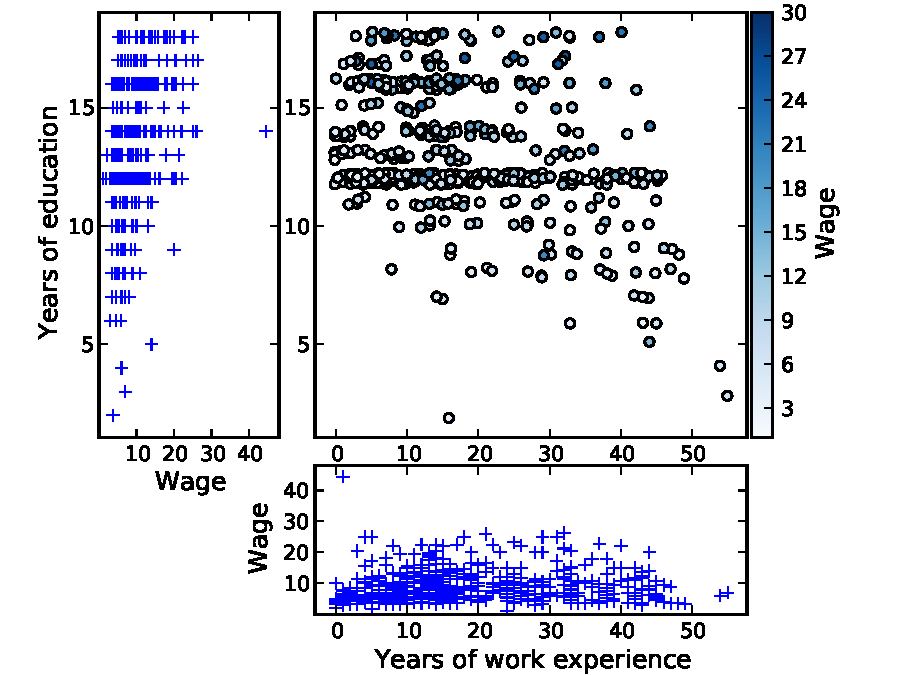
\includegraphics[width=1.05\linewidth]{wage_data}%

    \caption{Wage as a function of years of work experience and
    education; data from \cite{berndt1991}\label{fig:data}.}
\end{figure}

% Introduce and describe the data
Machine learning is about extracting rules from data, most often with the
goal of making decision on new data. As a simple example, we show on
Fig.\,\ref{fig:data} data about wages in the US, from \cite{berndt1991}:
11 features, including wage, number of years of education and of work
experience, on 534 individuals --samples in machine-learning
jargon. This data
Code downloading the data to reproduce the figures can be found on
\url{https://github.com/scikit-learn/SigMobile-paper}.
%
This data showcases many of the typical difficulties machine learning.
The samples are very irregularly distributed, as most individuals
finished their education after high-school. As a result, they are gapping
holes in the 2D plot education versus work experience, in which any
statistical analysis is extrapolation. The data is very noisy: for a
given education and work experience wages vary widely. This variability
can probably be explained with missing factors, such as sector of
activity, but adding them to the analysis creates a more complex picture,
in 3D or more, rather than 2D, with even more gaps.

On Fig.\,\ref{fig:random_forest}, we use a popular machine-learning
algorithm, Random Forests, to try to predict the wage from the years of
education, or the years of work experience, either as separate features,
or combined.

% Show an example of learning, first with random forest, and introduce
% overfit, then with svms, and discuss model complexity and use linear
% models to link to convention statistics. Conclude with the difference
% with 1D and 2D, and introduce the curse of dimensionality.
Discuss what we can learn from the wages examples. Introduce concepts of
overfitting, model complexity


\begin{figure}[b]
    %\hspace*{-.015\linewidth}%
    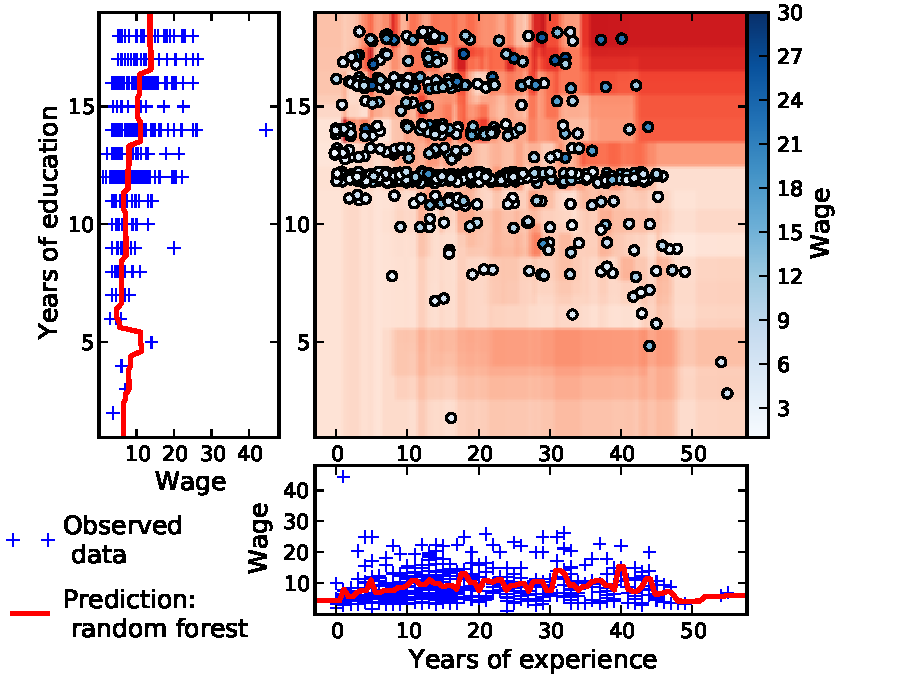
\includegraphics[width=1.05\linewidth]{wage_data_random_forest}%

    \caption{Wage prediction from years of work experience and education,
    using random forests.\label{fig:random_forest}}
\end{figure}

\begin{figure}[b]
    \hspace*{-.015\linewidth}%
    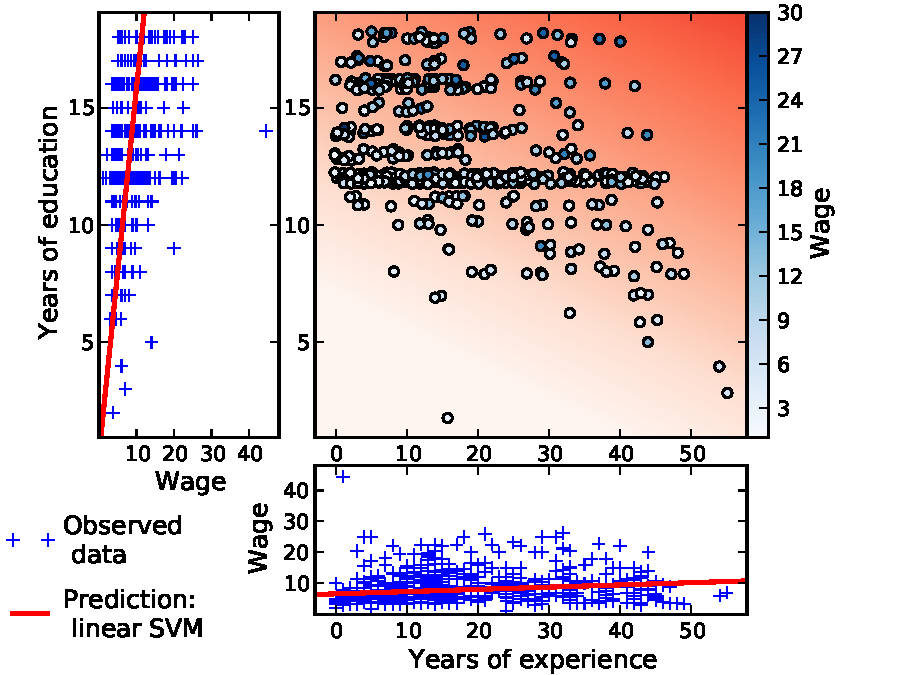
\includegraphics[width=1.05\linewidth]{wage_data_linear_svm}%

    \caption{Wage prediction from years of work experience and education,
    using a linear SVM.}
\end{figure}

\section{Learning with scikit-learn}

\paragraph{The data matrix}
%
Blahblah

\paragraph{Supervised models: learning to predict}
%
Blahblah

\paragraph{Model evaluation and parameter selection}
%
Model evaluation:
cross-validation: the concept, cross-val iterators, and cross\_val\_score

Problem of multiple metrics.

CV objects: GridSearchCV and RandomSearchCV, as well as FooBarCV objects.

\paragraph{Unsupervised models: learning to transform}
%
Unsupervised learning: a variety of usage pattern.

Many things can be seen as Transformers

Introduce the pipeline

\section{In practice}

\paragraph{A simple text-mining example}
%
% Lars: the following text presumes that NumPy, estimators, and the
% X/y convention for supervised learning have already been introduced.

Scikit-learn was designed around NumPy principles and data structures,
so virtually all estimators take arrays of numbers as input
and produce arrays as output.
That doesn't mean that it is limited to traditional number crunching domains,
though.
The library has been successfully employed in text classification
and natural language processing problems,
and utility code is provided to translate the unstructured, symbolic data
encountered in these domains
to the rigid matrix/vector structure that estimators expect.

In the NLP application domain,
features are typically 
where features are typically frequencies or boolean indicators
of very large numbers of rare events, such as
``document contains the term \textsf{v1agr@}'' (spam filtering)
or ``next token matches the Roman numeral regex'' (named-entity recognition).
To ensure scalability in the face of such data,
SciPy's sparse matrix data structures are supported by many estimators.\footnote{
  Support for these is added on a by-need basis,
  because using sparse data structures puts constraints on algorithm design
  and implementation.
}

The following example script is a fully functioning
sentiment polarity classifier for movie reviews:
given a review, it outputs the probability that the review is positive
about the movie it concerns.
The script demonstrates the use of pipelines,
and also shows how machine learning ties into Python's
``batteries included'' philosophy:
downloading, unpacking and learning from a dataset
are all done in one programming language.

% XXX make_pipeline is not in 0.14.1, we should release 0.15 sometime
% The example can be made a bit shorter by skipping the movie_reviews dir;
% the tarball from Pang et al. contain top-level cruft.
\begin{pythoncode}
import os.path
import tarfile
from urllib import urlretrieve
from sklearn.datasets import load\_files
from sklearn.feature\_extraction.text import TfidfVectorizer
from sklearn.linear\_models import LogisticRegression
from sklearn.pipeline import make\_pipeline

temp, \_ = urlretrieve('http://www.cs.cornell.edu/people/pabo/movie-review-data/review\_polarity.tar.gz')
with tarfile.open(temp) as tar:
    tar.extractall(path='movie\_reviews')
data = load\_files(os.path.join('movie\_reviews', 'txt\_sentoken'))

clf = make\_pipeline(TfidfVectorizer(min\_df=2, dtype=float,
                                    sublinear\_tf=True, ngram\_range=(1, 2),
                                    strip\_accents='unicode'),
                     LogisticRegression(random\_state=623, C=5000))
clf.fit(data.data, data.target)
\end{pythoncode}

This script first fetches the hand-labeled movie review dataset from
\cite{pang2004} and unpacks it to disk using standard Python libraries.
It then loads these into memory using the scikit-learn function
\texttt{load\_files}, makes a pipeline of a \textsf{tf--idf} feature extractor
\cite{rennie2003tackling} and logistic regression,
and finally trains the model.
The parameters for the feature extractor and the LogReg classifier
were tuned offline; the random-number generator seed is set by hand
to get reproducible results.

Does this classifier work?
We can find out by classifying some of our own movie reviews.\footnote{
  The code can be tried interactively by simply copy-pasting it
  into an interactive Python interpreter or IPython \cite{perez2007ipython}.
}

\begin{pythoncode}
>>> clf.predict\_proba(["This movie is the worst I ever saw.",
...                    "Shawshank Redemption, eat your heart out!"])
array([[  9.99293000e-01,   7.07000280e-04],
       [  1.68757754e-01,   8.31242246e-01]])
\end{pythoncode}

Here, we asked the model to predict the probability of a review being positive
for a batch of two reviews. It returns the negative probability in the first
column, the positive probability in the second.
As we can see, the first review gets a 99.9\% probability for being negative,
while the second has an 83\% probability of being positive.

Of course, that's just anecdotal evidence. We can get a figure for the
classifier's accuracy by retraining it in a five-fold cross-validation scheme:

\begin{pythoncode}
>>> from sklearn.cross\_validation import cross\_val\_score
>>> score = cross\_val\_score(clf, data.data, data.target, cv=5)
>>> score
array([ 0.91  ,  0.8825,  0.88  ,  0.8775,  0.86  ])
>>> score.mean()
0.88200000000000001
\end{pythoncode}

\paragraph{What about big data?}
%
Partial fit, random projections, HashingVectorizer

\section{Nurturing an open source project}

Goal: enable anybody to contribute, have a controlled process, grow.

Github, tests (link to travis)

Difficulty of getting credit, of rewarding properly the long tail of small
contributors, of finding funding. Problem of brain drain.

Difficulty of project scope (ideally: first cover all of statistical
learning classics \cite{elemstatlearn}) and default parameters

We have found that implementing, even a standard algorithm, really well,
can require a lot of domain knowledge. Thus it is natural that specific
libraries span up to solve it. Some adopt scikit-learn API and standard,
and we hope that scikit-learn has a structural effect on the environment.

Impact on education (documentation)

\small
\bibliography{paper}
\bibliographystyle{plain}


\end{document}
